\section{Methodological Framework: A Four-Stage Pipeline}
\label{sec:framework}

\begin{figure}[htbp]
    \centering
    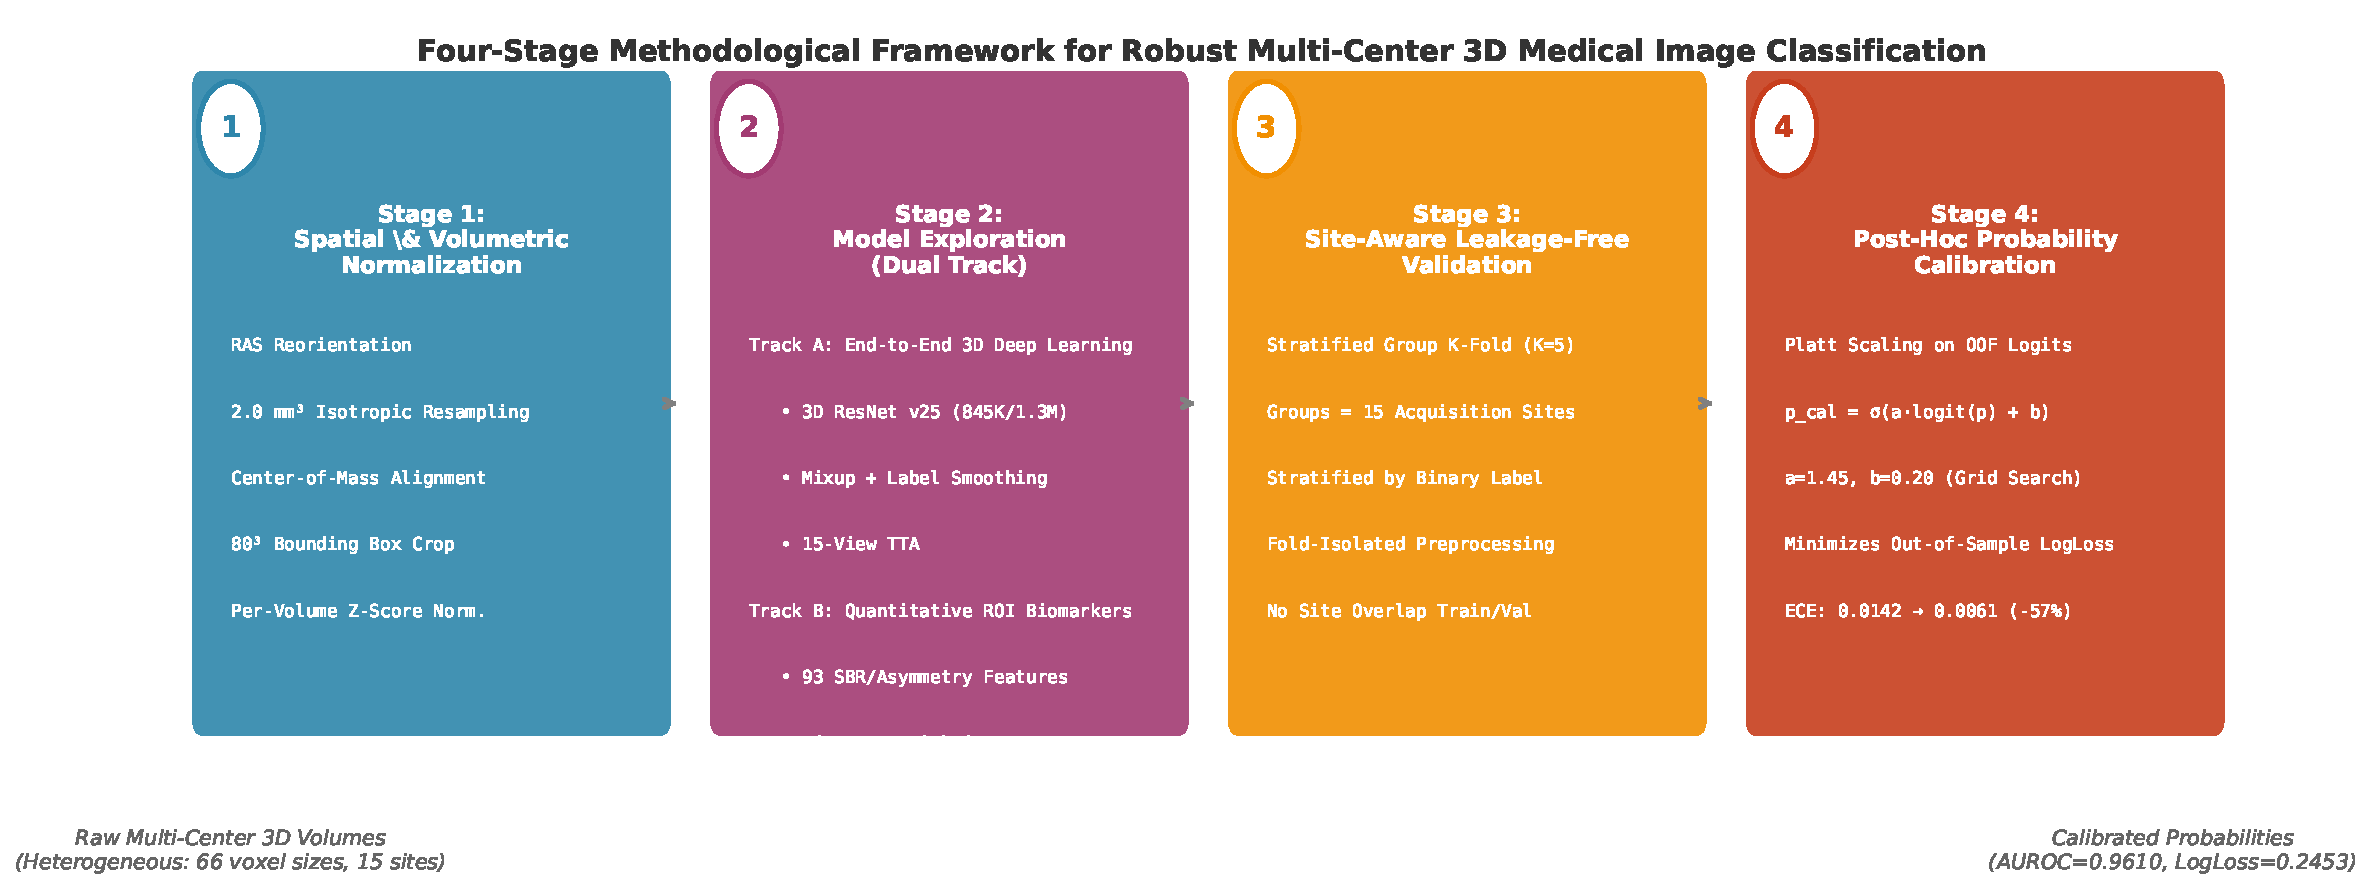
\includegraphics[width=0.95\linewidth]{figures/method_pipeline.pdf}
    \caption{The four-stage methodological framework for robust multi-center 3D medical image classification. Stage 1: Spatial \& volumetric normalization standardizes heterogeneous inputs. Stage 2: Model exploration compares end-to-end 3D deep learning against quantitative ROI biomarkers. Stage 3: Site-aware leakage-free validation ensures unbiased generalization estimates. Stage 4: Post-hoc probability calibration produces clinically reliable risk scores.}
    \label{fig:pipeline}
\end{figure}

Our framework decomposes the problem into four modular stages, each addressing a specific barrier to clinical deployment (Figure~\ref{fig:pipeline}).

\subsection{Stage 1: Spatial \& Volumetric Normalization}
\label{sec:framework_stage1}
Multi-center 3D scans arrive with heterogeneous voxel spacings (1.47--3.90~\voxelunit), matrix sizes (128--256), and slice counts (36--128). Stage 1 transforms all inputs into a canonical representation:
\begin{enumerate}
    \item \textbf{Reorientation:} Rigid affine transform to RAS (Right-Anterior-Superior) coordinate space using NIfTI affine metadata.
    \item \textbf{Isotropic Resampling:} Trilinear interpolation to 2.0~\voxelunit~isotropic voxels. Scaling factor per dimension: $f_i = \text{voxel}_i / 2.0$.
    \item \textbf{Center-of-Mass Alignment:} The COM of thresholded intensities ($>$5th percentile) is translated to the center of an $80^3$ grid (center = 39.5).
    \item \textbf{Per-Volume Z-Score Normalization:} $\tilde{v} = (v - \mu_v) / (\sigma_v + 10^{-8})$ computed independently per volume to prevent dataset-level statistics from leaking into validation.
    \item \textbf{Inference Normalization:} Intensity clipping to [1st, 99th] percentile, min-max scaling to [0, 1].
\end{enumerate}

This pipeline reduces 66 unique voxel sizes and 66 unique shapes to a uniform $80\times80\times80$ grid at 2.0~\voxelunit, preserving striatal signal across the full field-of-view.

\subsection{Stage 2: Model Exploration -- Dual Track}
\label{sec:framework_stage2}
We compare two complementary modeling paradigms:

\begin{description}
    \item[\textbf{Track A: End-to-End 3D Deep Learning.}] 3D ResNet variants with residual skip connections, three downsampling stages, and channel scaling (Net3dR-v25: 845K params; Net3dBig-v25: 1.3M params). Regularized by Mixup, label smoothing, and multi-view TTA.
    
    \item[\textbf{Track B: Quantitative ROI Biomarkers.}] Anatomically-guided feature extraction: striatal sub-regional intensity percentiles, hemispheric asymmetry indices, putamen-to-caudate ratios, and caudate-to-putamen gradients (93 features total). Modeled with gradient-boosted trees (XGBoost, LightGBM) and linear models.
\end{enumerate}

This dual-track design directly tests whether learned 3D representations outperform expert-engineered clinical biomarkers.

\subsection{Stage 3: Site-Aware Leakage-Free Validation}
\label{sec:framework_stage3}
Naive random cross-validation leaks scanner-site signatures because scans from the same site share acquisition characteristics. We formalize \cvname:

\begin{equation}
    \mathcal{D}_{\text{train}}, \mathcal{D}_{\text{val}} = \text{StratifiedGroupKFold}(\mathcal{D}, \text{groups}=\text{site\_id}, n_{\text{splits}}=5)
\end{equation}

where groups are the 15 acquisition centers. This ensures no scanner appears in both training and validation within any fold, providing an unbiased estimate of generalization to unseen sites. All preprocessing statistics (normalization, feature selection) are computed fold-isolated.

\subsection{Stage 4: Post-Hoc Probability Calibration}
\label{sec:framework_stage4}
Raw cross-entropy training produces overconfident models (ECE=0.0142). Stage 4 applies Platt scaling on out-of-fold ensemble logits:

\begin{equation}
    p_{\text{cal}} = \sigma(a \cdot z + b) = \frac{1}{1 + \exp(-(a \cdot \text{logit}(p) + b))}
\end{equation}

where $z = \text{logit}(p) = \log(p / (1-p))$, and parameters $(a,b)$ are fit by minimizing LogLoss on OOF predictions via grid search. This minimizes out-of-sample LogLoss while preserving AUROC, yielding clinically reliable risk estimates.